% !TEX program = lualatex
\documentclass[11pt]{article}

% -------- LuaLaTeX : polices et langue --------
\usepackage{fontspec}
\setmainfont{Latin Modern Roman}
\setsansfont{Tex Gyre Heros}
%\renewcommand{\familydefault}{\sfdefault} % force le sans serif par défaut
\usepackage{polyglossia}
\setdefaultlanguage{french}

% -------- Mise en page --------
\usepackage[a4paper,margin=1cm]{geometry}
\usepackage{multicol}
\usepackage{fancyhdr}
\pagestyle{empty}
\usepackage[most]{tcolorbox}

% -------- Mathématiques --------
\usepackage{amsmath,amssymb,mathtools}
% \usepackage{siunitx}
% \sisetup{locale=FR}

\usepackage{enumitem}
\setlist[itemize]{left=0pt}
\setlist[enumerate]{left=0pt, label=\textbf{\alph*}.}

\usepackage{ProfCollege}
\usepackage{ProfMaquette}

%\usepackage{tabularray}
\usepackage{tabularx}

% -------- Divers --------
\newcommand{\ligne}{{\color{gray!60}\hrulefill}}

\setlength{\parindent}{0pt}

\begin{document}



\begin{Maquette}[IE]{
        Numero = 1, Code={}, Date = Jeudi 14 octobre, Theme = Géométrie / Automatismes, Calculatrice = false
    }

    \begin{exercice}
        \brm{3} Ci-dessous, trace l’image du quadrilatère CDEF par la translation qui transforme A en B.
        \begin{center}
            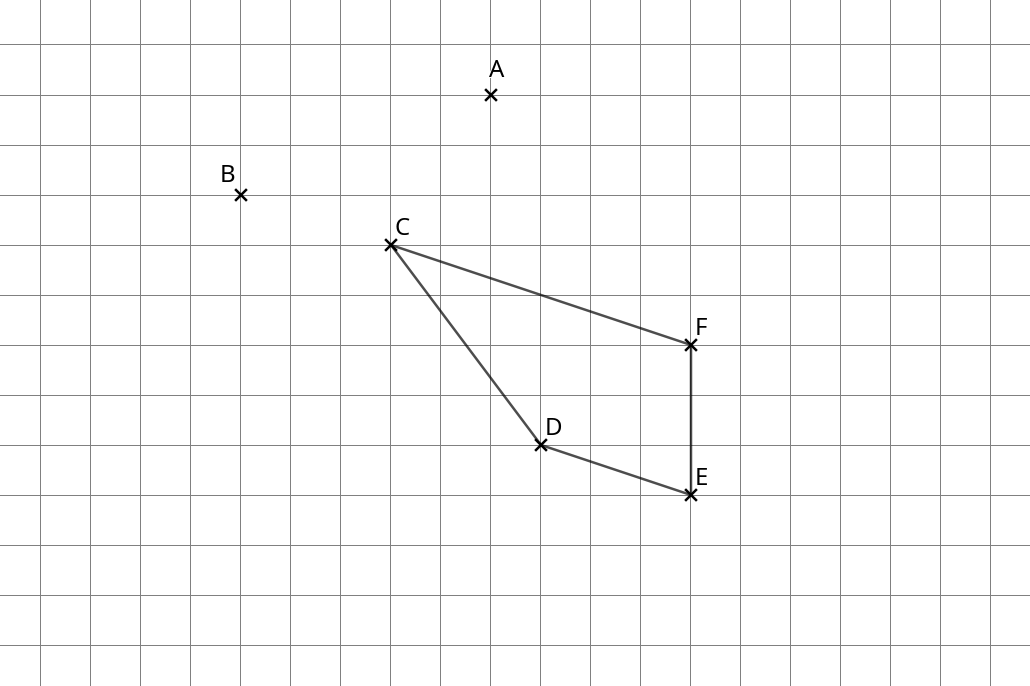
\includegraphics[width = .85 \linewidth]{Images/Évaluation 2 - Translation.png}
        \end{center}
    \end{exercice}

    \vspace{.5cm}
    \begin{exercice}
        \begin{multicols}{2}
            \begin{center}
                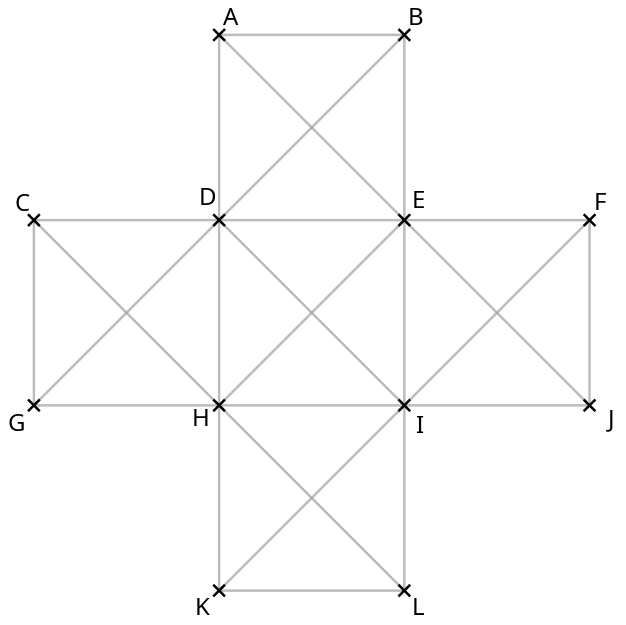
\includegraphics[width = \linewidth]{Images/Évaluation 2 - Croix.png}
            \end{center}
            \columnbreak
            Donne l’image du triangle HIL par …
            \begin{enumerate}[itemsep=5pt]
                \brm{4}
                \item la translation qui transforme I en D ? \ligne
                \item la translation qui transforme L en E ? \ligne
                \item la translation de vecteur $\overrightarrow{CA}$ ? \ligne
                \item la translation de vecteur $\overrightarrow{DC}$ ? \ligne
            \end{enumerate}
        \end{multicols}
    \end{exercice}

    \newpage

    \begin{exercice}
        \brm{3}
        \begin{center}
            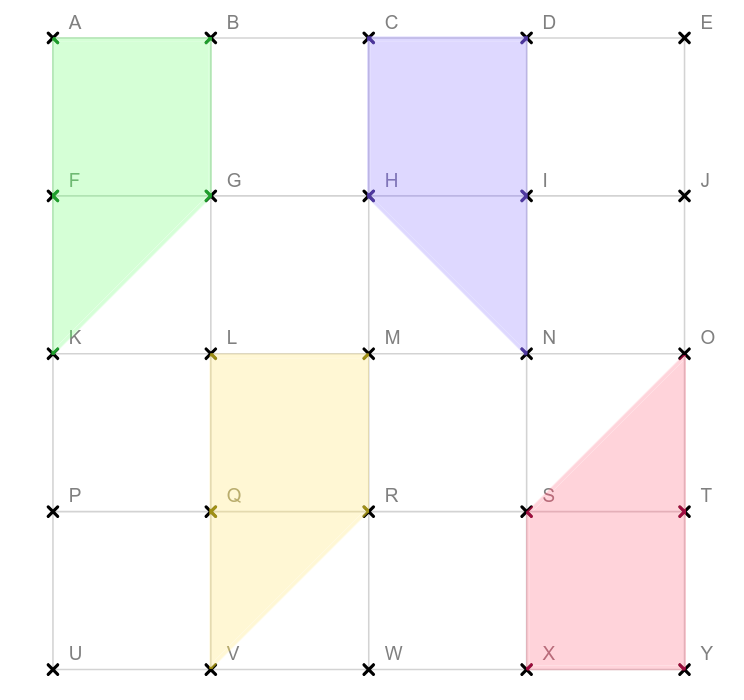
\includegraphics[width=.65\linewidth]{Images/Évaluation 2 - Quadrillage.png}
        \end{center}
        {\small
        \begin{tabularx}{\textwidth}{X|X|X}
            DCHN est l’image de ABGK par …

            \begin{itemize}[label=$\square$, itemsep=10pt, topsep=10pt]
                \item une translation
                \item une symétrie axiale
                \item une symétrie centrale
            \end{itemize}

                                    &

            LMRV est l’image de ABGK par …

            \begin{itemize}[label=$\square$, itemsep=10pt, topsep=10pt]
                \item une translation
                \item une symétrie axiale
                \item une symétrie centrale
            \end{itemize}

                                    &
            YXSO est l’image de ABGK par …

            \begin{itemize}[label=$\square$, itemsep=10pt, topsep=10pt]
                \item une translation
                \item une symétrie axiale
                \item une symétrie centrale
            \end{itemize}
        \end{tabularx}
        }
    \end{exercice}

    \vspace{.5cm}
    \begin{exercice}
        \begin{multicols}{2}
            \begin{itemize}[itemsep=10pt]
                \brm{5}
                \item le triple de $4$ : \ligne
                \item la moitié de $13$ : \ligne
                \item le carré de $11$ : \ligne
                \item le tiers de $60$ : \ligne
                \item le double de $2,4$ : \ligne
                \item $2,4 \times 100$ : \ligne
                \item $1789 \div 1000$ : \ligne
                \item $7 \div 100$: \ligne
                \item $21 \times 1000$ : \ligne
                \item $750 \div 10$ : \ligne
                \item $4-10$: \ligne
                \item $-2-5$: \ligne
                \item $-7+1$: \ligne
                \item $-5+15$: \ligne
                \item $5 - (-2)$: \ligne
                \item écriture réduite de $3 \times x \times 2 $ : \ligne
                \item écriture réduite de $3 x + 2$ : \ligne
                \item écriture réduite de $a \times 5 \times a$: \ligne
                \item écriture réduite de $5a - 6a$: \ligne
                \item écriture réduite de $a+2b+4a$: \ligne
            \end{itemize}
        \end{multicols}
    \end{exercice}
\end{Maquette}


\end{document}